% !TeX spellcheck = en_EN
% !TeX encoding = UTF-8
% !TeX program = xelatex
%----------------------------------------------------------------------------
\chapter{Implementation}
%----------------------------------------------------------------------------

This section provides an in-depth explanation of the code generator's architecture and implementation. First, it begins with the requirements of the code generator itself, then section 4.2 delves into the specifics of the results after generation. Following that, section 4.3 explores the architecture and design used within the project. Lastly, the chapter concludes with a discussion on the current limitations of the code generator, highlighting any known constraints or areas for future improvement.

%----------------------------------------------------------------------------
\section{Requirements}
%----------------------------------------------------------------------------

The C code generator reuse architectural and design patterns from
the already existing Java code generator\cite{Gamma} of Gamma. Though the two languages are very different, they both have to provide the same functionalities to correctly implement a component.

Each generated implementations must be able to:
\begin{itemize}
	\item Initialize, reset the component
	\item Execute a step on the component
	\item Reset in-, outputs between steps
\end{itemize}

The following section presents the architecture that made the aforementioned demands possible. 

%----------------------------------------------------------------------------
\section{C Code Generation}
%----------------------------------------------------------------------------

Within the generated code, Gamma components are implemented as C structs, while regions are represented as an enums. Initializations, resets, and transitions, which define the behavior and state changes of the system, are implemented as functions.

Unlike object-oriented languages such as Java, C does not provide built-in support for interfaces, classes, or namespaces. The absence of the aforementioned features poses a challenge when attempting to apply modular code organization in C development. To overcome these limitations, the C code generator take advantage of the fact that two components cannot have the same in XSTS. While this approach works for regions and components, there is a possibility that states within different regions cause conflicts. To solve yet another problem connected to the absence of namespaces, the adoption of a specific naming convention is required. By appending the name of the region after each state having an underscore between, we have the solution we needed.
\bigskip

\begin{lstlisting}[language=C, caption={Representation of the Main Region in C}]
	/* Enum representing region Main_region_Controller */
	enum Main_Region_Controller {
		__Inactive___main_region_controller,
		Operating_main_region_controller,
		Interrupted_main_region_controller
	} main_region_controller;
\end{lstlisting}

The generation of necessary functions is carried out similarly to the generation of regions. The main difference between the two conventions is the appendix. In case of functions and routines, we append the name of the component to which it belongs.
\bigskip

\begin{lstlisting}[language=C, caption={Function declarations in C}]
	/* Reset component Crossroad */
	void resetCrossroadStatechart(CrossroadStatechart* statechart);
	/* Initialize component Crossroad */
	void initializeCrossroadStatechart(CrossroadStatechart* statechart);
	/* Entry event of component Crossroad */
	void entryEventsCrossroadStatechart(CrossroadStatechart* statechart);
	/* Clear input events of component Crossroad */
	void clearInEventsCrossroadStatechart(CrossroadStatechart* statechart);
	/* Clear output events of component Crossroad */
	void clearOutEventsCrossroadStatechart(CrossroadStatechart* statechart);
	/* Transitions of component Crossroad */
	void changeStateCrossroadStatechart(CrossroadStatechart* statechart);
	/* Run cycle in component Crossroad */
	void runCycleCrossroadStatechart(CrossroadStatechart* statechart);
\end{lstlisting}

Introducing a wrapper statechart, as an extra layer above the component, is essential as it handles timing, abstracts internal mechanisms, and provides ports for interaction. The C language does not support encapsulation in the form of private attributes, therefore the user can interact with the component directly despite the fact that the code is meant to be hidden. Through ports, it enables controlled access to internal state and data. These ports were realized as setters / getters for the ease of use. By managing timing-related behaviors, it ensures the independence of our layers, one being the component itself which is responsible for the internal mechanism, while the responsibilities of the wrapper component were already summarized.

%----------------------------------------------------------------------------
\section{Structure of the Code Generator}
%----------------------------------------------------------------------------

The structure of the code generator consists of several packages and classes. In the main directory, the \textit{IStatechartCode} interface is provided, which serves as the contract for each source and header file pair. The \textit{CodeBuilder} class implements this interface and is responsible for constructing the source and header files for the components. Similarly, the \textit{WrapperBuilder} class also implements the \textit{IStatechartCode} interface and is responsible for building the wrapper source and header files.

Within the model package, there are two models and a common abstract base. The \textit{FileModel} class is the latter that handles file related operations. The \textit{CodeModel} class represents the model for the source code files, while the \textit{HeaderModel} class represents the model for the header files.

\begin{figure}[h]
	\centering
	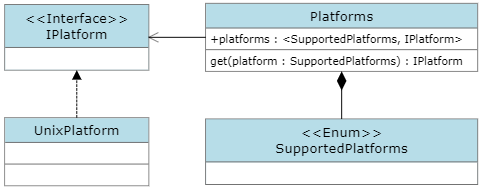
\includegraphics[width=0.8\textwidth]{images/platforms.png}
	\caption{The structure of the platforms package.}
	\label{fig:timing}
\end{figure}

The platforms package is specifically designed for platform-independent timing code generation. It contains the \textit{IPlatform} interface, which is required by each platform implementation. At the end of this semester there is only one supported platform:

\begin{itemize}
	\item Unix Platform
\end{itemize}

The serializer package plays a vital role in serializing various components of the XSTS models into C code. It includes the \textit{ActionSerializer} class, which serializes actions into C code, the \textit{ExpressionSerializer} class for serializing expressions, the \textit{TypeDeclarationSerializer} class for serializing type declarations into C enums, and the \textit{VariableDeclarationSerializer} class, which serializes variable declarations into C code, potentially within the component struct.

%----------------------------------------------------------------------------
\section{Current Limitations}
%----------------------------------------------------------------------------

The code generator has certain limitations that should be considered. For instance, it does not provide support for all types of gamma compositions, such as any asynchronous composition. Additionally, it is currently limited to Unix platforms, which may restrict its usage in certain environments. Moreover, the precision which we measure elapse time with also acts as a limiting factor. The model stores clock values as integers in milliseconds. Its granularity may not be sufficient for all applications that require more precise timing. Rounding errors may occur when converting between different units, leading to potential inaccuracies. Additionally, the code generator relies on variables to track elapsed time. In certain scenarios, if the elapsed time exceeds the maximum value that can be stored in the certain variable type, in our case an unsigned integer, an overflow may occur. This can lead to unexpected behavior or even segmentation faults in the generated code.
